% Made up for the tikra benchmark.
% White light through a prism, spread into its colors.
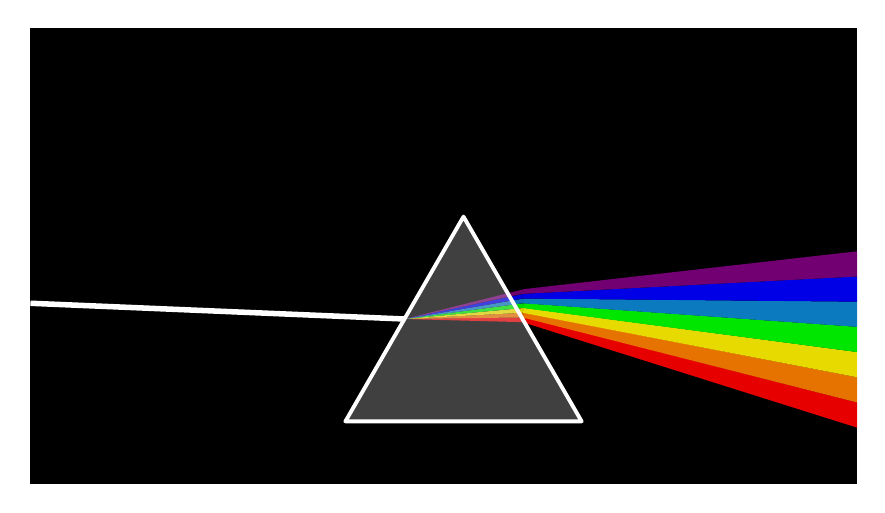
\begin{tikzpicture}
  \fill[black] (-4,-2.4) rectangle (6.5,3.4);
  \coordinate (A) at (0,-1.6); \coordinate (B) at (3,-1.6); \coordinate (C) at (1.5,1.0);
  \draw[white, line width=2pt] (-4,-0.1) -- (0.75,-0.3);
  \foreach \c/\o [count=\i] in {red/0.55, orange/0.45, yellow/0.35, green/0.22, cyan!70!blue/0.12, blue/0.0, violet/-0.1} {
    \fill[\c, opacity=0.85] (0.75,-0.3) -- (2.25,-0.4+0.06*\i) -- (2.27,-0.4+0.06*\i+0.06) -- cycle;
    \fill[\c, opacity=0.9] (2.25,-0.4+0.06*\i) -- (6.5,-2.0+0.32*\i) -- (6.5,-2.0+0.32*\i+0.32) -- (2.27,-0.4+0.06*\i+0.06) -- cycle;
  }
  \fill[white, opacity=0.25] (A) -- (B) -- (C) -- cycle;
  \draw[white, line width=1.4pt, line join=round] (A) -- (B) -- (C) -- cycle;
\end{tikzpicture}
